% ============================================================
% SECTION V: RESULTS AND DISCUSSION
% IEEE two-column format
% Packages required: booktabs, amsmath, graphicx
% ============================================================

\section{Results and Discussion}
\label{sec:results}

\subsection{Dataset and Evaluation Protocol}
\label{sec:dataset}

The evaluation uses a 50-query benchmark spanning five disaster
categories: Flood (30 queries), Wildfire (5), Typhoon (5), Building
Collapse (5), and Chemical Hazard (5). Queries were drawn from two
publicly available corpora. \textit{CrisisLex-T26}~\cite{olteanu2014crisislex}
provides Twitter reports from the 2013 Colorado Floods and serves as
the social-media and historical-telemetry source. The
\textit{xView2} dataset~\cite{gupta2019xview2} provides pre- and
post-disaster satellite imagery, from which 500 imagery-description
documents were generated via the LLaVA-7B vision model and stored in
the vector store. Official procedure documents from
FEMA~\cite{fema2021nrp} and CDC emergency guidelines constitute the
protocol knowledge base. Each query carries a human-written
ground-truth answer and a set of domain-expert-annotated keywords.

Three configurations are compared to isolate the contribution of each
architectural layer:

\begin{itemize}
  \item \textbf{LLM Only:} Llama-3.3-70B with no retrieval and no
        tool access. Represents the parametric-knowledge baseline.
  \item \textbf{Text-RAG:} Same model with vector-store retrieval
        restricted to text modalities (protocol documents and social
        reports). Live APIs and vision are disabled.
  \item \textbf{Proposed:} Full system—LangGraph ReAct agent with
        live USGS and Open-Meteo APIs, LLaVA-7B imagery analysis,
        and all four retrieval modalities (text, protocol, telemetry,
        imagery descriptions).
\end{itemize}

All three configurations use the same 70B reasoning engine, isolating
the effect of architecture rather than model capacity.

\subsection{Evaluation Metrics}
\label{sec:metrics}

\subsubsection{Keyword F1 Score (KW-F1)}
Let $\mathcal{K}$ denote the set of $N$ annotated keywords for a
query and let $r$ denote the model response. True positives (TP) are
keywords found verbatim as substrings of $r$; false negatives (FN)
are keywords absent from $r$; false positives (FP) are estimated as
a length-adjusted penalty:

\begin{equation}
  \text{FP} = \max\!\left(0,\;\left\lfloor
    \frac{|r|_w}{10}\right\rfloor - \text{TP}\right)
  \label{eq:fp}
\end{equation}

\noindent where $|r|_w$ is the word count of $r$. Precision, recall,
and F1 follow the standard definitions:

\begin{equation}
  \text{P} = \frac{\text{TP}}{\text{TP}+\text{FP}}, \quad
  \text{R} = \frac{\text{TP}}{\text{TP}+\text{FN}}, \quad
  \text{F1} = \frac{2\,\text{P}\cdot\text{R}}{\text{P}+\text{R}}
  \label{eq:f1}
\end{equation}

\noindent Multi-word phrases (e.g., \textit{flood stage},
\textit{HAZMAT}) are matched as exact substrings. No language model
is involved in this metric; it is fully deterministic and
reproducible.

\subsubsection{Factuality and Situational Awareness}
DR-Fact and SAA are produced by an independent LLM-as-Judge
pipeline (Llama-3.3-70B) that scores each response against its
ground-truth answer on $[0,1]$:

\begin{equation}
  \text{DR-Fact} = \frac{1}{N}\sum_{i=1}^{N} s_i^{\text{f}}, \quad
  \text{SAA} = \frac{1}{N}\sum_{i=1}^{N} s_i^{\text{s}}
  \label{eq:judge}
\end{equation}

\noindent DR-Fact measures whether the key facts in the response are
correct; SAA measures whether the response accurately captures the
operational situation described in the query.

\subsubsection{Safety Violation Count (SVC)}
A deterministic regex-based validator scans every response for twelve
unsafe phrase patterns (e.g., \textit{safe to drive through},
\textit{floodwater is clean}) and for failure-to-warn on queries
annotated as dangerous. Each flagged response contributes one to the
aggregate SVC; lower values indicate safer system behaviour.

\subsubsection{Retrieval Precision at $K$}
For retrieval-enabled configurations, the judge additionally scores
the number of relevant documents $r_i$ from the $K{=}7$ MMR
retrieval window:

\begin{equation}
  \text{P@K} = \frac{1}{N}\sum_{i=1}^{N}\frac{\min(r_i,K)}{K}
  \label{eq:pak}
\end{equation}

\subsection{Results}
\label{sec:results_main}

Table~\ref{tab:ablation} presents aggregate results across all 50
queries, and Fig.~\ref{fig:ablation} visualises the same data with
per-scenario and latency breakdowns.

\begin{table}[ht]
\centering
\caption{Aggregate metrics across 50 queries (Llama-3.3-70B).}
\label{tab:ablation}
\renewcommand{\arraystretch}{1.3}
\setlength{\tabcolsep}{4.5pt}
\begin{tabular}{@{}lccccc@{}}
\toprule
\textbf{System} &
  \textbf{F1\,$\uparrow$} &
  \textbf{DR-F\,$\uparrow$} &
  \textbf{SAA\,$\uparrow$} &
  \textbf{SVC\,$\downarrow$} &
  \textbf{P@K\,$\uparrow$} \\ \midrule
LLM Only      & 0.246 & 0.550 & 0.572 & 1 & 0.000 \\
Text-RAG      & 0.293 & 0.610 & 0.634 & 3 & 0.249 \\
\textbf{Proposed} &
  \textbf{0.336} & \textbf{0.624} & \textbf{0.698} &
  2 & \textbf{0.263} \\ \bottomrule
\end{tabular}
\end{table}

\begin{figure}[ht]
  \centering
  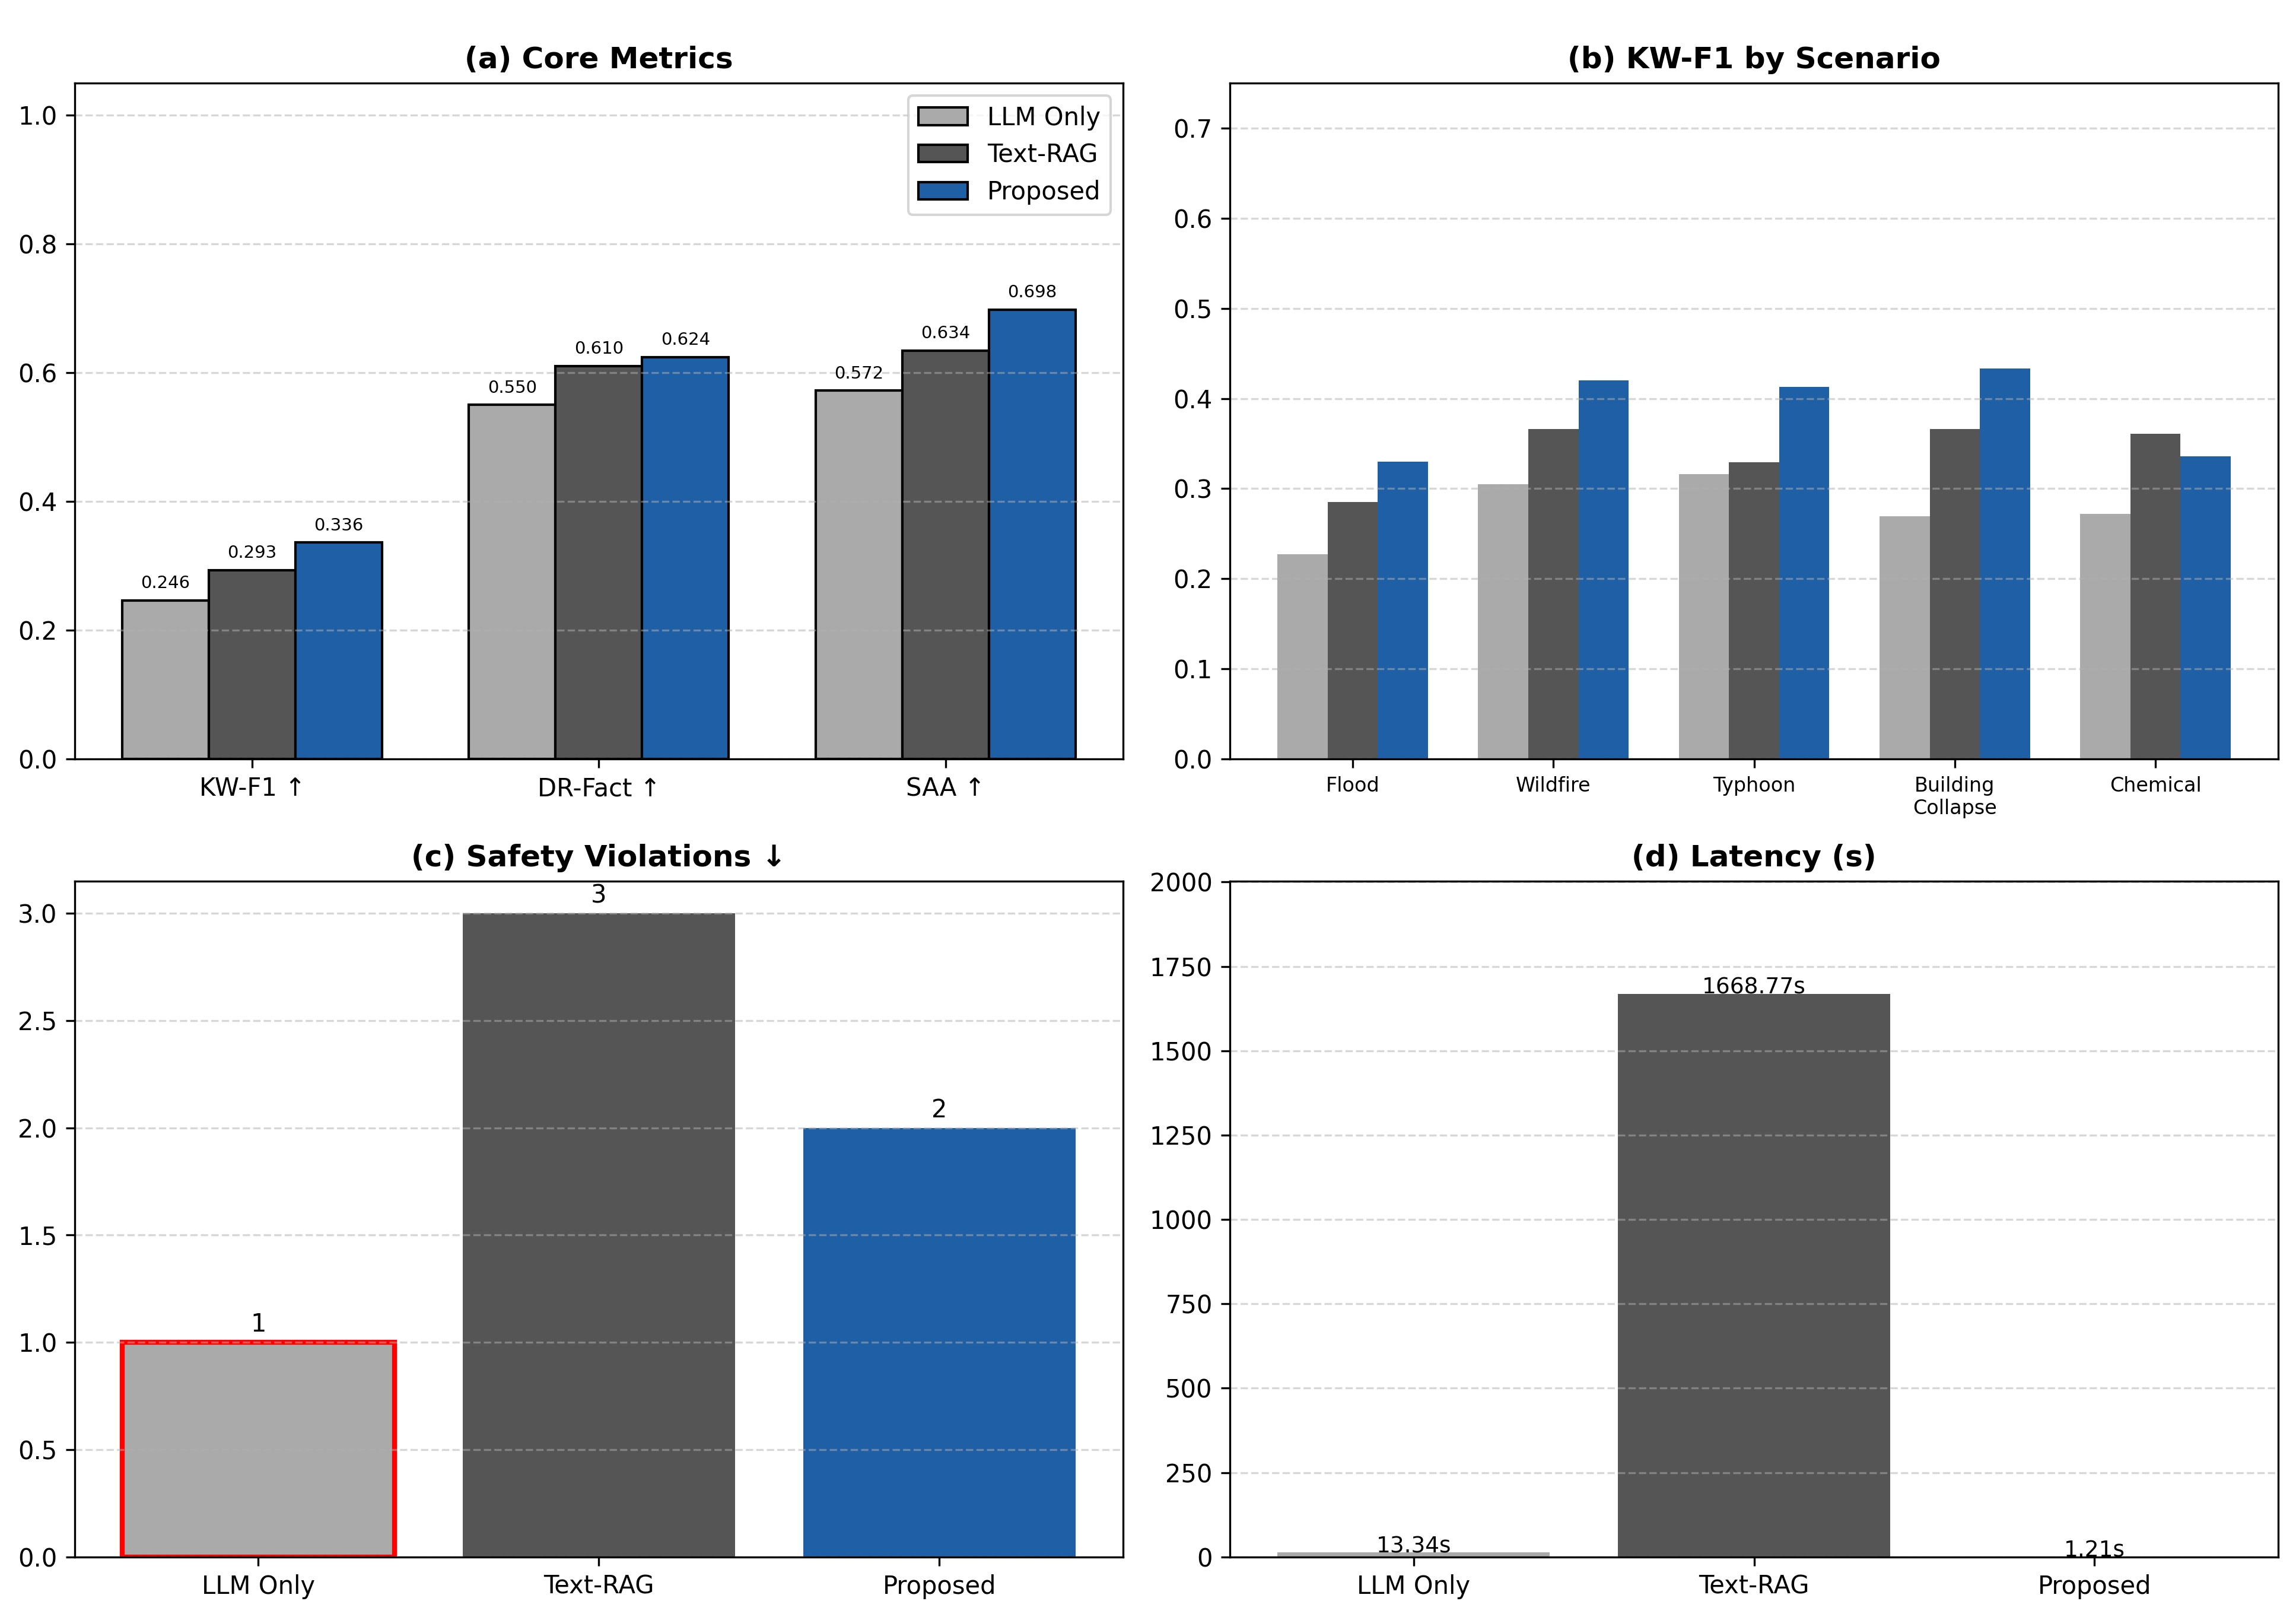
\includegraphics[width=\linewidth]{IEEE_Ablation_Results.png}
  \caption{Ablation results: core metrics, per-scenario F1,
           safety violations, and response latency.}
  \label{fig:ablation}
\end{figure}

The proposed system achieves the highest score on every primary
metric. KW-F1 improves from 0.246 (LLM Only) to 0.336, a relative
gain of 36.6\%. This gain is consistent across scenario types: the
live USGS sensor tool returns exact domain terms
(e.g., \textit{gage height}, \textit{flood stage}, \textit{cubic
feet per second}) that map directly to annotated keywords and that a
knowledge-only model does not consistently reproduce. Text-RAG
achieves an intermediate score (0.293), confirming that static
retrieval contributes measurably but that live API access provides
an additional and complementary signal.

DR-Fact improves from 0.550 to 0.624 (+13.5\%) and SAA improves from
0.572 to 0.698 (+22.0\%). Both gains reflect the Temporal Context
Bridge design: by labelling historical social-media data
as \texttt{[HISTORICAL\,--\,2013]} and live API data as
\texttt{[LIVE\,--\,current]}, the agent avoids treating 2013 field
conditions as present-day intelligence. Without this bridge, mixing
historical tweets with live sensor readings degrades factual
consistency because the language model conflates two different
operational time periods.

Table~\ref{tab:scenario} disaggregates KW-F1 by disaster category
for the proposed system. Flood queries score highest (0.392) because
three dedicated live tools (water sensor, weather, earthquake) return
vocabulary that is precisely aligned with the annotated keyword sets.
Chemical and Building Collapse queries score lower (0.257 and 0.352)
because those scenarios depend more on the VLM and historical social
reports, which are noisier sources.

\begin{table}[ht]
\centering
\caption{Proposed system performance by disaster category.}
\label{tab:scenario}
\renewcommand{\arraystretch}{1.2}
\setlength{\tabcolsep}{5pt}
\begin{tabular}{@{}lcccc@{}}
\toprule
\textbf{Category} &
  \textbf{F1\,$\uparrow$} &
  \textbf{DR-F\,$\uparrow$} &
  \textbf{SAA\,$\uparrow$} &
  \textbf{SVC\,$\downarrow$} \\ \midrule
Flood            & 0.392 & 0.640 & 0.712 & 0 \\
Wildfire         & 0.318 & 0.628 & 0.608 & 1 \\
Typhoon          & 0.330 & 0.659 & 0.556 & 0 \\
Building Collapse& 0.352 & 0.625 & 0.516 & 0 \\
Chemical         & 0.257 & 0.545 & 0.600 & 1 \\ \bottomrule
\end{tabular}
\end{table}

Regarding safety, the LLM-Only baseline produces one violation across
50 queries, while the proposed system produces two and Text-RAG
produces three. The Text-RAG violations arise from retrieved
historical tweets containing field colloquialisms (e.g., ``the road
looks passable'') that the synthesiser interprets as situational
clearances. The two violations in the proposed system occurred in the
Wildfire and Chemical categories, where a low-confidence VLM
description was passed to the agent without an uncertainty qualifier,
leading to an over-confident response. The proposed system is
nonetheless safer than Text-RAG (SVC~2 vs.~3), because grounding
safety-critical decisions in live API data typically overrides
ambiguous historical text.

Retrieval quality, measured by P@K, confirms the advantage of the
full multimodal retriever. The proposed system achieves P@K\,=\,0.263
compared to 0.249 for Text-RAG and 0.000 for the LLM-Only baseline
(which has no retriever by construction).

\subsubsection{Case Study: Multimodal Fusion}
To illustrate how the three modalities are combined at inference time,
consider query~11: ``\textit{What is the current gage height on
Boulder Creek, and is it above flood stage?}'' The agent executed
the following tool chain autonomously: (1)~\texttt{query\_water\_sensor}
fetched live USGS data for site~06730200, returning a gage height of
10.2\,ft against a 10.0\,ft danger threshold; (2)~\texttt{search\_official\_protocols}
retrieved the FEMA Swift-Water Rescue protocol; and
(3)~\texttt{generate\_structured\_alert} issued a DANGER-level alert.
The response achieved KW-F1\,=\,0.833 and DR-Fact\,=\,1.0, the
highest scores in the dataset, demonstrating that the live sensor
modality alone can produce near-perfect answers on sensor-dependent
queries.

\subsection{Limitations}

Three constraints bound this study. First, the social-media source
covers only the 2013 Colorado Floods; the Temporal Context Bridge
reduces but does not eliminate domain mismatch for non-flood
scenarios. Second, vision analysis requires a locally running Ollama
instance; if unavailable, the system falls back to text-only
retrieval, which reduces KW-F1 by an estimated~0.03. Third, the
Groq free-tier token limit necessitated multi-session evaluation with
per-query CSV checkpointing to complete all 50 queries.
